\pdfoutput=1
\documentclass[11pt]{article}
\usepackage{jheppub}
\usepackage{epsfig}
\usepackage{amssymb}
\usepackage{amsmath}
\usepackage{tikz}
\usepackage{mathrsfs}
\usepackage{hyperref}
\usepackage{multirow}
\usepackage{scalerel}
\usepackage{mathtools}
\usepackage{MnSymbol}
\usepackage[all]{xy}

\usetikzlibrary{calc}


\DeclareMathOperator{\B}{B}
\DeclareMathOperator{\Conf}{Conf}
\DeclareMathOperator{\Gr}{Gr}
\DeclareMathOperator{\Gl}{Gl}
\DeclareMathOperator{\Li}{Li}
\DeclareMathOperator{\sgn}{sgn}


\def\ket#1{\langle #1 \rangle}
\def\nl{\nonumber\\}
\def\nn{\nonumber}
\def\x{\mathcal{X}}
\def\a{\mathcal{A}}
\def\draftnote#1{{\bf [#1]}}

\def\drawPentagon{
\coordinate (P1) at (90:1);
\coordinate (P2) at (18:1);
\coordinate (P3) at (306:1);
\coordinate (P4) at (234:1);
\coordinate (P5) at (162:1);
\draw (P1) -- (P2) -- (P3) -- (P4) -- (P5) -- cycle;
}

\def\drawLabeledPentagon{
\coordinate (P1) at (90:1);
\coordinate (P2) at (18:1);
\coordinate (P3) at (306:1);
\coordinate (P4) at (234:1);
\coordinate (P5) at (162:1);
\draw (P1) -- (P2) -- (P3) -- (P4) -- (P5) -- cycle;
\draw (0,1.2) node {1};
\draw (1,.3) node[anchor=west] {2};
\draw (.5,-.9) node[anchor=west] {3};
\draw (-.5,-.9) node[anchor=east] {4};
\draw (-1,.3) node[anchor=east] {5};
}

\def\drawOctagon{
\coordinate (P1) at (45:1);
\coordinate (P2) at (90:1);
\coordinate (P3) at (135:1);
\coordinate (P4) at (180:1);
\coordinate (P5) at (225:1);
\coordinate (P6) at (270:1);
\coordinate (P7) at (315:1);
\coordinate (P8) at (359:1);
\draw (P1) -- (P2) -- (P3) -- (P4) -- (P5) -- (P6) -- (P7) -- (P8) -- cycle;
}

\title{A Physicist's Introduction to Cluster Algebras, with Applications to Polylogarithms and Amplitudes}

\author{John~Golden}


\affiliation{Leinweber  Center for Theoretical Physics and
Randall Laboratory of Physics, Department of Physics,
University of Michigan
Ann Arbor, MI 48109, USA}

\abstract{We give a quick and schematic introduction to cluster algebras with an emphasis on examples and applications over mathematical background. Most of this material was introduced to the amplitudes literature in \cite{ArkaniHamed:2012nw} and \cite{Golden:2013xva}, which focused on applications at integrand and integrated amplitudes, respectively. However I have found that these introductory sources are written at a level of mathematical rigour which can make them difficult to parse for the reader looking for a first introduction to the subject. This is a particular shame since cluster algebras are much like chess: the rules are simple to learn yet take a lifetime to master. My hope with this introduction is to give a quick introduction to the most elemental facts about cluster algebras and work through some simple examples. There are unfortunately many beautiful topics and applications left unmentioned. }

\begin{document}
\maketitle

\section{Introduction}
Cluster algebras were introduced by Fomin and Zelevinsky \cite{1021.16017}, in large part motivated by questions of total positivity. The original goal was to gain a better understanding of what algebraic varieties can have a natural notion of positivity, and what functions can determine such positivity. A simple and highly-relevant example for amplitudes is the positive Grassmannian $\Gr^+(k,n)$, i.e. the space of $k\times n$ matrices where all ordered $k\times k$ minors are positive. 

Before I further describe what a cluster algebra is, let me give a more precise idea of what questions cluster algebras help us answer. One very nice question that we can gain some handle on is: how many minors do we need to specify a point in $\Gr^+(k,n)$? In other words, given a $k \times n$ matrix $M$, how many minors of $M$ do we have to calculate to know if $M \in \Gr^+(k,n)$? The reason that this is an interesting question is that the minors are not all independent, they satisfy identities known as Pl\"ucker relations:
\begin{equation}
  \label{eq:plucker-rel}
  \ket{abI} \ket{cdI} = \ket{acI} \ket{bdI} + \ket{adI}\ket{bcI},
\end{equation}
where the Pl\"ucker coordinates = $\ket{i_1,\ldots,i_k}$ = the minor of columns $i_1, \ldots,i_k$, and $I$ is a multi-index with $k-2$ entries.

Let's work through the example of $\Gr(2,5)$ in detail to try to understand how many minors one needs to check for positivity of the whole matrix. First of all, we'll definitely have to check the 5 cyclically adjacent minors, $\ket{12}, \ket{23}, \ket{34}, \ket{45}, \ket{15}> 0$, as they are all independent from each other. Now, how many of the non-adjacent minors do we have to check? It turns out that the answer is 2. For example, if we specify that $\ket{13}, \ket{14}>0$ then we can use Pl\"ucker relations to show
\begin{equation}
\begin{split}
	\ket{24} &= (\ket{12}\ket{34} + \ket{23}\ket{14})/\ket{13}\\
	\ket{25} &= (\ket{12}\ket{45} + \ket{24}\ket{15})/\ket{14}\\
	\ket{35} &= (\ket{25}\ket{34} + \ket{23}\ket{45})/\ket{24}.
\end{split}	 	
\end{equation} 
Here we have expressed all of the remaining minors as sums and products of the cyclically adjacent minors along with $\ket{13}$ and $\ket{14}$, so everything is positive. 

So we only need to check two -- but can we check any two? Clearly we can use any of the cyclic images of $\{\ket{13}, \ket{14}\}$. What about $\{\ket{13}, \ket{25}\}$? This is a bit harder to see, but no, this pair does not work: there is no way to write down the remaining Pl\"uckers in terms of $\ket{13}$ and $\ket{25}$ such that everything is manifestly positive. For example, the matrix
\begin{equation}
\left(
\begin{array}{ccccc}
 1 & -1 & -4 & 3 & -2 \\
 2 & 2 & -6 & 4 & -1 \\
\end{array}
\right)
\end{equation}
satisfies $\ket{12},\ldots,\ket{15},\ket{13},\ket{25}>0$ but has $\ket{14}<0$. In the end, $\{\ket{13}, \ket{14}\}$ and its cyclic images are the only pairs that describe a point in $\Gr^+(2,5)$. 

This was easy enough to work out for this small case, but I think it is also easy to convince yourself that the problem gets much more complicated for larger matrices. However, there is a closely related, and much simpler, problem in geometry which can give us a bit more intuition: triangulating polygons.

Consider the following triangulation of the pentagon:
\begin{equation}
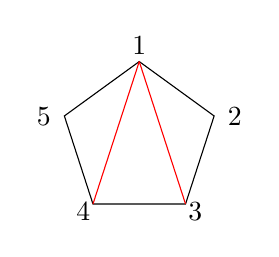
\begin{tikzpicture}
  \drawLabeledPentagon
  \draw[color=red] (P1) -- (P3);
  \draw[color=red] (P1) -- (P4);
\end{tikzpicture}
\end{equation}
We can immediately see the parallels with our $\Gr(2,5)$ situation (this is an example of the more general Pl\"ucker embedding which connects $\Gr(k,n)$ with projective space). Here we associate lines connecting points $i$ and $j$ with the Pl\"ucker coordinate $\ket{ij}$, and we see that the triangulations of the pentagon all describe points in $\Gr^+(2,5)$. In fact this correspondence holds between $n$-gons and $\Gr(2,n)$. 

A simple observation, but one at the very heart of cluster algebras, is that given some triangulation of a polygon one can create a \emph{new} triangulation by picking a quadrilateral and flipping its diagonal. For example:
\begin{equation}
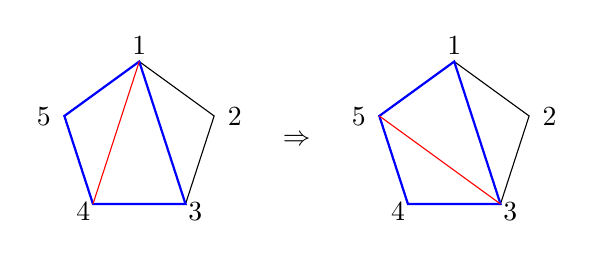
\begin{tikzpicture}
  \drawLabeledPentagon
  \draw[color=blue, thick] (P1) -- (P3) -- (P4) -- (P5) -- cycle;
  \draw[color=red] (P1) -- (P4);
  \draw (2,0) node {$\Rightarrow$};
\begin{scope}[xshift = 4cm]
  \drawLabeledPentagon
  \draw[color=blue, thick] (P1) -- (P3) -- (P4) -- (P5) -- cycle;
  \draw[color=red] (P5) -- (P3);
\end{scope}
\end{tikzpicture} 
\end{equation}
By repeatedly performing these flips one can generate all possible triangulations of a polygon:\pagebreak
\begin{figure}[h]
  \centering
  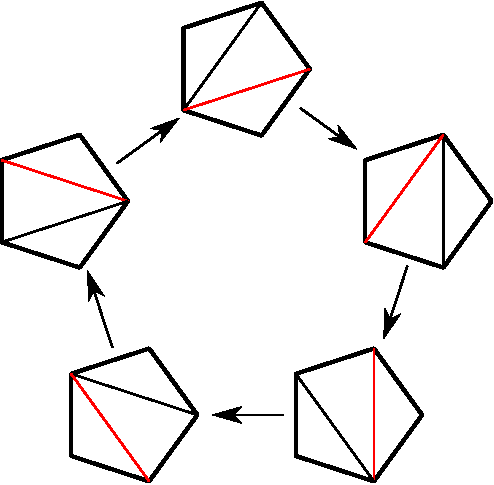
\includegraphics[scale=0.6]{pentagon-triangulations}
\end{figure}

\noindent where in each case the red diagonal gets flipped. 

Cluster algebras are a combinatorial tool which captures all of this structure (and much more!). The basic idea is that a cluser algebra is a collection of \emph{clusters}, which in this case represent individual triangulations of an $n$-gon, and these clusters are connected via a process called \emph{mutation}, which in this case is the flipping-the-diagonal process. I will initially describe everything in terms of Grassmannian cluster algebras, but the framework is entirely generalizable to other contexts of interest.

\section{Basic definition}

Let's construct the cluster algebra for $\Gr(2,5)$. Each cluster is labeled by a collection of coordinates, which in this case are the edges of our pentagon along with the diagonals of the particular triangulation. These coordinates are then connected via an orientation of the pentagon and all subtriangles, for example:
\begin{equation}\label{eq:oriented-pentagon}
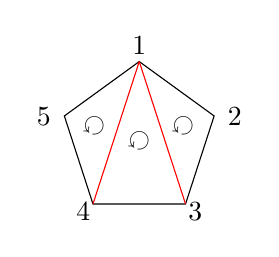
\begin{tikzpicture}
  \drawLabeledPentagon
  \draw[color=red] (P1) -- (P3);
  \draw[color=red] (P1) -- (P4);
  \draw (18:.6) node[rotate=144] {$\circlearrowleft$};
  \draw (0:0) node[rotate=144] {$\circlearrowleft$};
  \draw (162:.6) node[rotate=144] {$\circlearrowleft$};
\end{tikzpicture} 
\end{equation}
We can redraw this diagram as
\begin{equation}\label{eq:gr25-seed}
\begin{gathered}
\begin{xy} 0;<1pt,0pt>:<0pt,-1pt>::
	(25,25) *+{\langle 13\rangle} ="0",
	(75,25) *+{\langle 14\rangle} ="1",
	(125,25) *+{\framebox[5ex]{$\langle 15\rangle$}} ="2",
	(125,75) *+{\framebox[5ex]{$\langle 45\rangle$}} ="3",
	(75,75) *+{\framebox[5ex]{$\langle 34\rangle$}} ="4",
	(25,75) *+{\framebox[5ex]{$\langle 23\rangle$}} ="5",
	(0,0) *+{\framebox[5ex]{$\langle 12\rangle$}} ="6",
	(145,75) *+{},
	"0", {\ar"1"},
	"4", {\ar"0"},
	"0", {\ar"5"},
	"6", {\ar"0"},
	"1", {\ar"2"},
	"3", {\ar"1"},
	"1", {\ar"4"},
\end{xy}
\end{gathered}
\end{equation}
In this quiver diagram, we have an arrow between two Pl\"uckers $\ket{ab} \to \ket{cd}$ if the triangle orientations in eq. (\ref{eq:oriented-pentagon}) have segment $(ab)$ flowing into segment $(cd)$. The boxes around the $\ket{ii+1}$ indicate that they are \emph{frozen} -- in other words, we never change the outer edges of the pentagon, only the diagonal elements. And lastly it is unnecessary to draw the arrows connecting the outer edges, as that is redundant (and unchanging) information. 

We have now drawn our first cluster (also sometimes called a seed). To review/introduce some terminology, the Pl\"uckers are called cluster $\a$-coordinates (sometimes also $\a$-variables), and they come in two flavors: mutable ($\ket{13}$ and $\ket{14}$) and frozen ($\ket{ii+1}$). The information of the arrows can be represented in terms of a skew-symmetric adjacency matrix
\begin{equation}
	b_{i j} = (\# \text{arrows}\; i \to j) - (\# \text{arrows}\; j \to i).
\label{eq:bijdef}
\end{equation}

The process of mutation, which we described geometrically in terms of flipping the diagonal, has a simple interpretation at the level of this quiver. In particular, given a quiver such as eq. (\ref{eq:gr25-seed}), chose a node $k$ with associated $\a$-coordinate $a_k$ to mutate on (this is equivalent to picking which diagonal to flip). Then draw a new quiver that changes $a_{k}$ to $a_{k}'$ defined by
\begin{equation}
  \label{eq:mutation}
  a_{k} a_{k}' = \prod_{i \vert b_{i k} > 0} a_{i}^{b_{i k}} + \prod_{i \vert b_{i k} < 0} a_{i}^{-b_{i k}},
\end{equation} (with the understanding that an empty product is set to one) and leaves the other cluster coordinates unchanged. The arrows connecting the nodes in this new cluster are modified from the original cluster according to
\begin{itemize}
	\item for each path $i\to j \to k$, add an arrow $i\to j$,
	\item reverse all arrows on the edges incident with $k$,
	\item and remove any two-cycles that may have formed.
\end{itemize}
This creates a new adjacency matrix $b_{ij}'$ via 
\begin{equation}
  \label{eq:b-mutation}
  b'_{i j} =
  \begin{cases}
    -b_{i j}, &\quad \text{if $k \in \lbrace i, j\rbrace$,}\\
    b_{i j}, &\quad \text{if $b_{i k} b_{k j} \leq 0$,}\\
    b_{i j} + b_{i k} b_{k j}, &\quad \text{if $b_{i k}, b_{k j} > 0$,}\\
    b_{i j} - b_{i k} b_{k j}, &\quad \text{if $b_{i k}, b_{k j} < 0$.}
  \end{cases}
\end{equation}
Mutation is an involution, so mutating on $a_k'$ will take you back to the original cluster (as flipping the same diagonal twice will take you back to where you started). 

For our purposes, \emph{a cluster algebra is a set of quivers closed under mutation}. This means that mutating on any node of any quiver will generate a different quiver in the cluster algebra. The general procedure is to start with a quiver such as eq. (\ref{eq:gr25-seed}), with some collection of frozen and unfrozen variables in a connected quiver, and continue mutating on all available nodes until you either close your set or convince yourself that the cluster algebra is infinite. 

\section{Finiteness and Grassmannian cluster algebras}

What cluster algebras are finite? Fomin and Zelevinksy \cite{1054.17024} showed that a cluster algebra is of finite type iff the mutable part of its quiver at some cluster takes the form of an oriented, simply-laced Dynkin diagram:
\begin{figure}[h!]
  \centering
  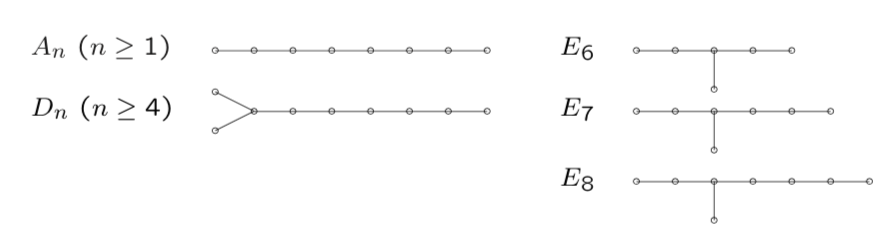
\includegraphics[scale=0.4]{finite-types.png}
\end{figure}

\noindent Looking back at eq. (\ref{eq:gr25-seed}), we see that the mutable nodes take the form of an $A_2$ Dynkin diagram. For this reason, we often speak of the $\Gr(2,5)$ and $A_2$ cluster algebras interchangeably. More broadly, we have the correspondence 
\begin{equation}
	\text{triangulations of an $n$-gon}\leftrightarrow \Gr(2,n) \text{ cluster algebra} \leftrightarrow A_{n-3} \text{ Dynkin diagram.}
\end{equation}
And for $\Gr(k,n)$, Scott showed \cite{1088.22009} that the associated seed cluster is
\begin{center}
\begin*{}
\begin{xy} 0;<.5pt,0pt>:<0pt,-.5pt>::
(0,0) *+{f_{1 l}} ="0",
(75,0) *+{\cdots} ="1",
(150,0) *+{f_{13}} ="2",
(225,0) *+{f_{12}} ="3",
(300,0) *+{\framebox[5ex]{$f_{11}$}} ="4",
(0,75) *+{f_{2 l}} ="5",
(75,75) *+{\cdots} ="6",
(150,75) *+{f_{23}} ="7",
(225,75) *+{f_{22}} ="8",
(300,75) *+{\framebox[5ex]{$f_{21}$}} ="9",
(0,150) *+{\vdots} ="10",
(75,150) *+{\vdots} ="11",
(150,150) *+{\vdots} ="12",
(225,150) *+{\vdots} ="13",
(300,150) *+{\vdots} ="14",
(0,225) *+{\framebox[5ex]{$f_{kl}$}} ="15",
(75,225) *+{\cdots} ="16",
(150,225) *+{\framebox[5ex]{$f_{k3}$}} ="17",
(225,225) *+{\framebox[5ex]{$f_{k2}$}} ="18",
(300,225) *+{\framebox[5ex]{$f_{k1}$}} ="19",
(-60,0) *+{} ="20",
"0", {\ar"1"},
"0", {\ar"5"},
"6", {\ar"0"},
"1", {\ar"2"},
"2", {\ar"3"},
"2", {\ar"7"},
"8", {\ar"2"},
"3", {\ar"4"},
"3", {\ar"8"},
"9", {\ar"3"},
"5", {\ar"6"},
"5", {\ar"10"},
"6", {\ar"7"},
"7", {\ar"8"},
"7", {\ar"12"},
"13", {\ar"7"},
"8", {\ar"9"},
"8", {\ar"13"},
"14", {\ar"8"},
"10", {\ar"15"},
"12", {\ar"17"},
"19", {\ar"13"},
"18", {\ar"12"},
"13", {\ar"18"},
\end{xy}
\end*{}
\end{center}

\noindent where
\begin{equation}
  f_{i j} =
  \begin{cases}
    \frac {\langle i+1, \dotsc, k, k+j, \dotsc, i+j+k-1\rangle}{\langle 1, \dotsc, k\rangle}, \qquad &i \leq l-j+1,\\
    \frac {\langle 1, \dotsc, i+j-l-1, i+1, \dotsc, k, k+j, \dotsc, n\rangle}{\langle 1, \dotsc, k\rangle}, \qquad &i > l-j+1
  \end{cases},
\end{equation}
We can use this to find the Grassmannian cluster algebras of finite type, they are:
\begin{equation}
	\Gr(2,n) \leftrightarrow A_{n-3}, \quad \Gr(3,6) \leftrightarrow D_4, \quad \Gr(4,7) \leftrightarrow E_6, \quad \Gr(3,8) \leftrightarrow E_8.
\end{equation}
An intriguing point for those of us studying $\mathcal{N}=4$ SYM, where the momentum twistors describing particle kinematics live in $\Gr(4,n)$, is that only $\Gr(4,n<8)$ are finite. The ramifications of the fact that $n>7$-particle kinematics are associated with infinite cluster algebras are still being worked out. 

\section{Associahedra}

Understanding the way in which clusters are related to each other via mutation is a hot topic of research. A sample question is: given two clusters in the same cluster algebra, what is the minimal set of mutations necessary to get from one cluster to the other? While I don't delve in to this area too much, I do want to give an introduction to a relevant and important object associated with a cluster algebra: the associahedron (often also called the Stasheff polytope). The basic idea is to create a graph where the nodes are clusters and edges are drawn between clusters connected via mutation. So the figure
\begin{figure}[h]
  \centering
  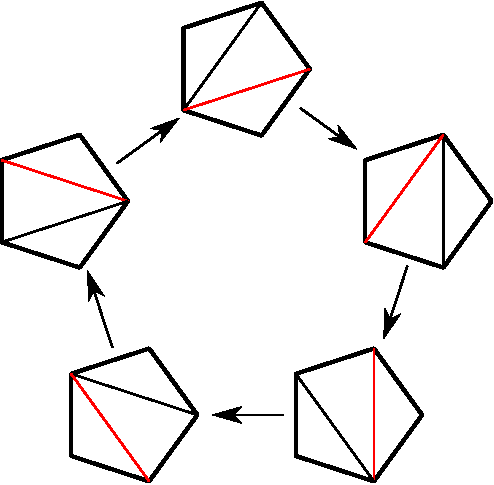
\includegraphics[scale=0.6]{pentagon-triangulations}
\end{figure}

\noindent is in fact the $\Gr(2,5)$ or $A_2$ associahedron, and clearly it takes the form of a pentagon (one should ignore the orientation on the edges of the pentagon).

The associahedron associated with the $\Gr(2,6) \leftrightarrow A_3$ cluster algebra (i.e. triangulations of a hexagon) is
\begin{figure}[h]
  \centering
  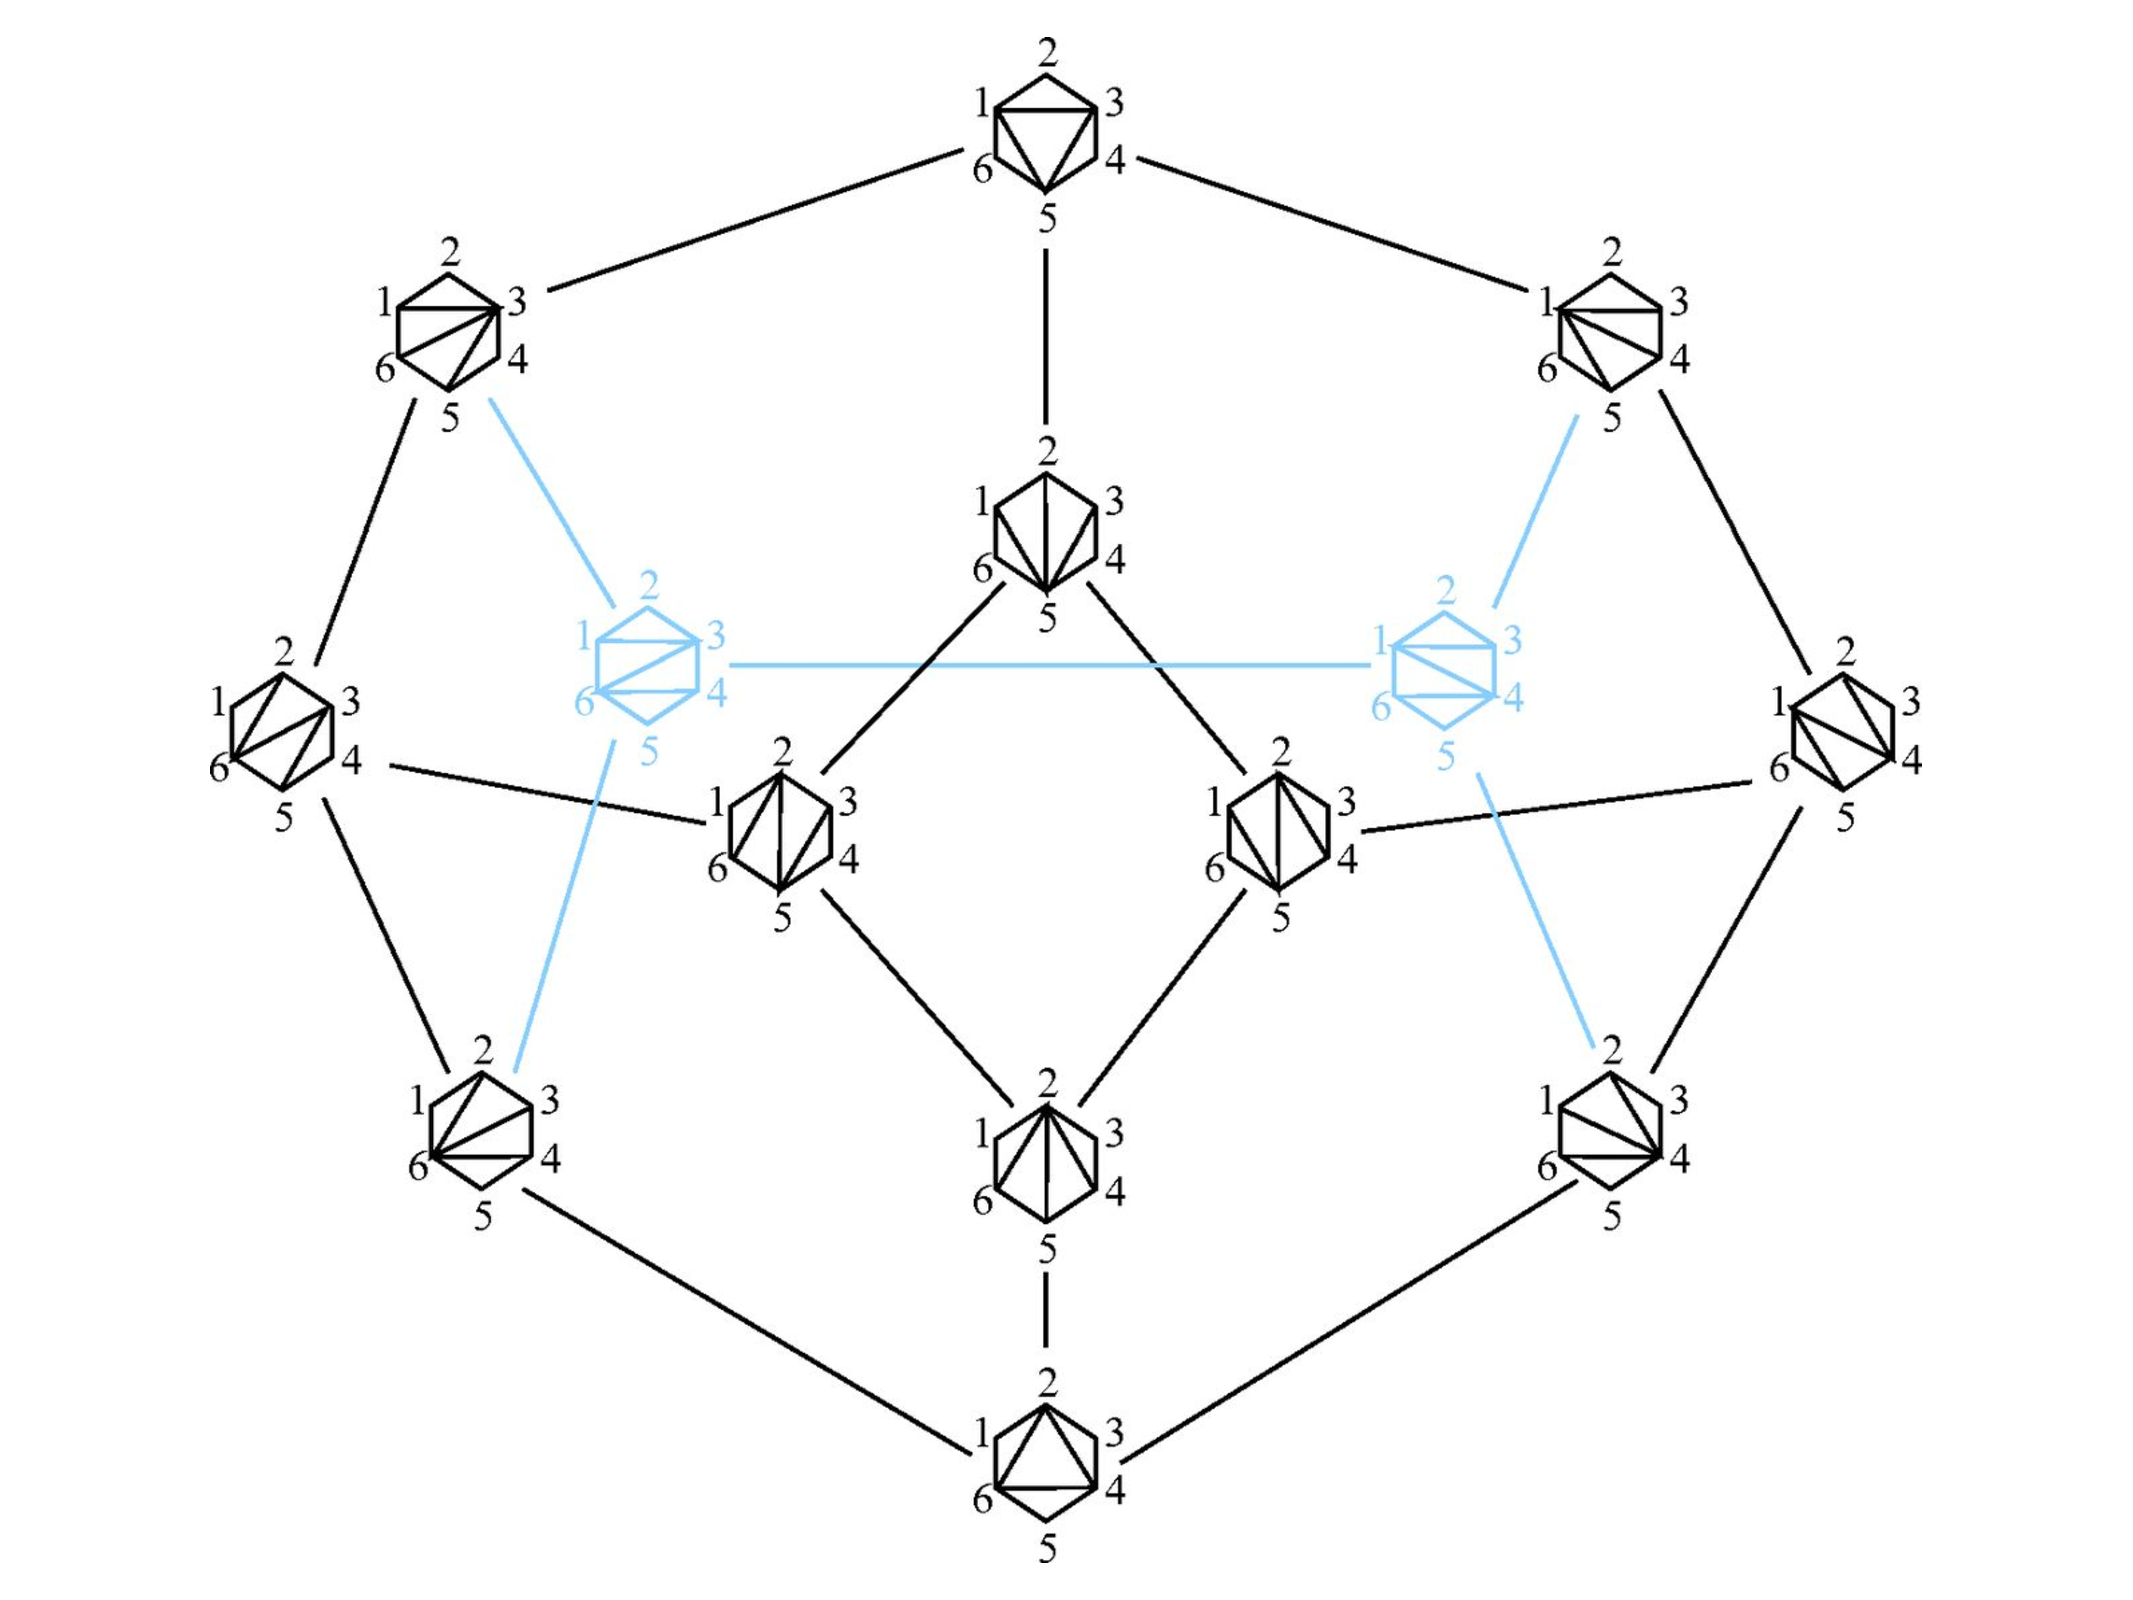
\includegraphics[scale=0.25]{a3-associahedron}
\end{figure}

\noindent This associahedron has 14 vertices, with 3 square faces and 6 pentagonal faces. Because of the Grassmannian duality $\Gr(2,6) = \Gr(4,6)$, this (remarkably simple!) cluster algebra and associahedron play an integral role in the momentum twistors for 6-particle kinematics for $\mathcal{N}=4$ SYM. 

$\Gr(4,7) \leftrightarrow E_6$, which is associated with 7-particle momentum twistors, is a bit more complicated: it features 833 clusters, and the associahedron is a polytope with nodes of valence 6. The dimension-2 faces are 1785 squares and 1071 pentagons, and there are 49 different $A$-coordinates that appear. The associahedron looks like
\begin{figure}[h]
  \centering
  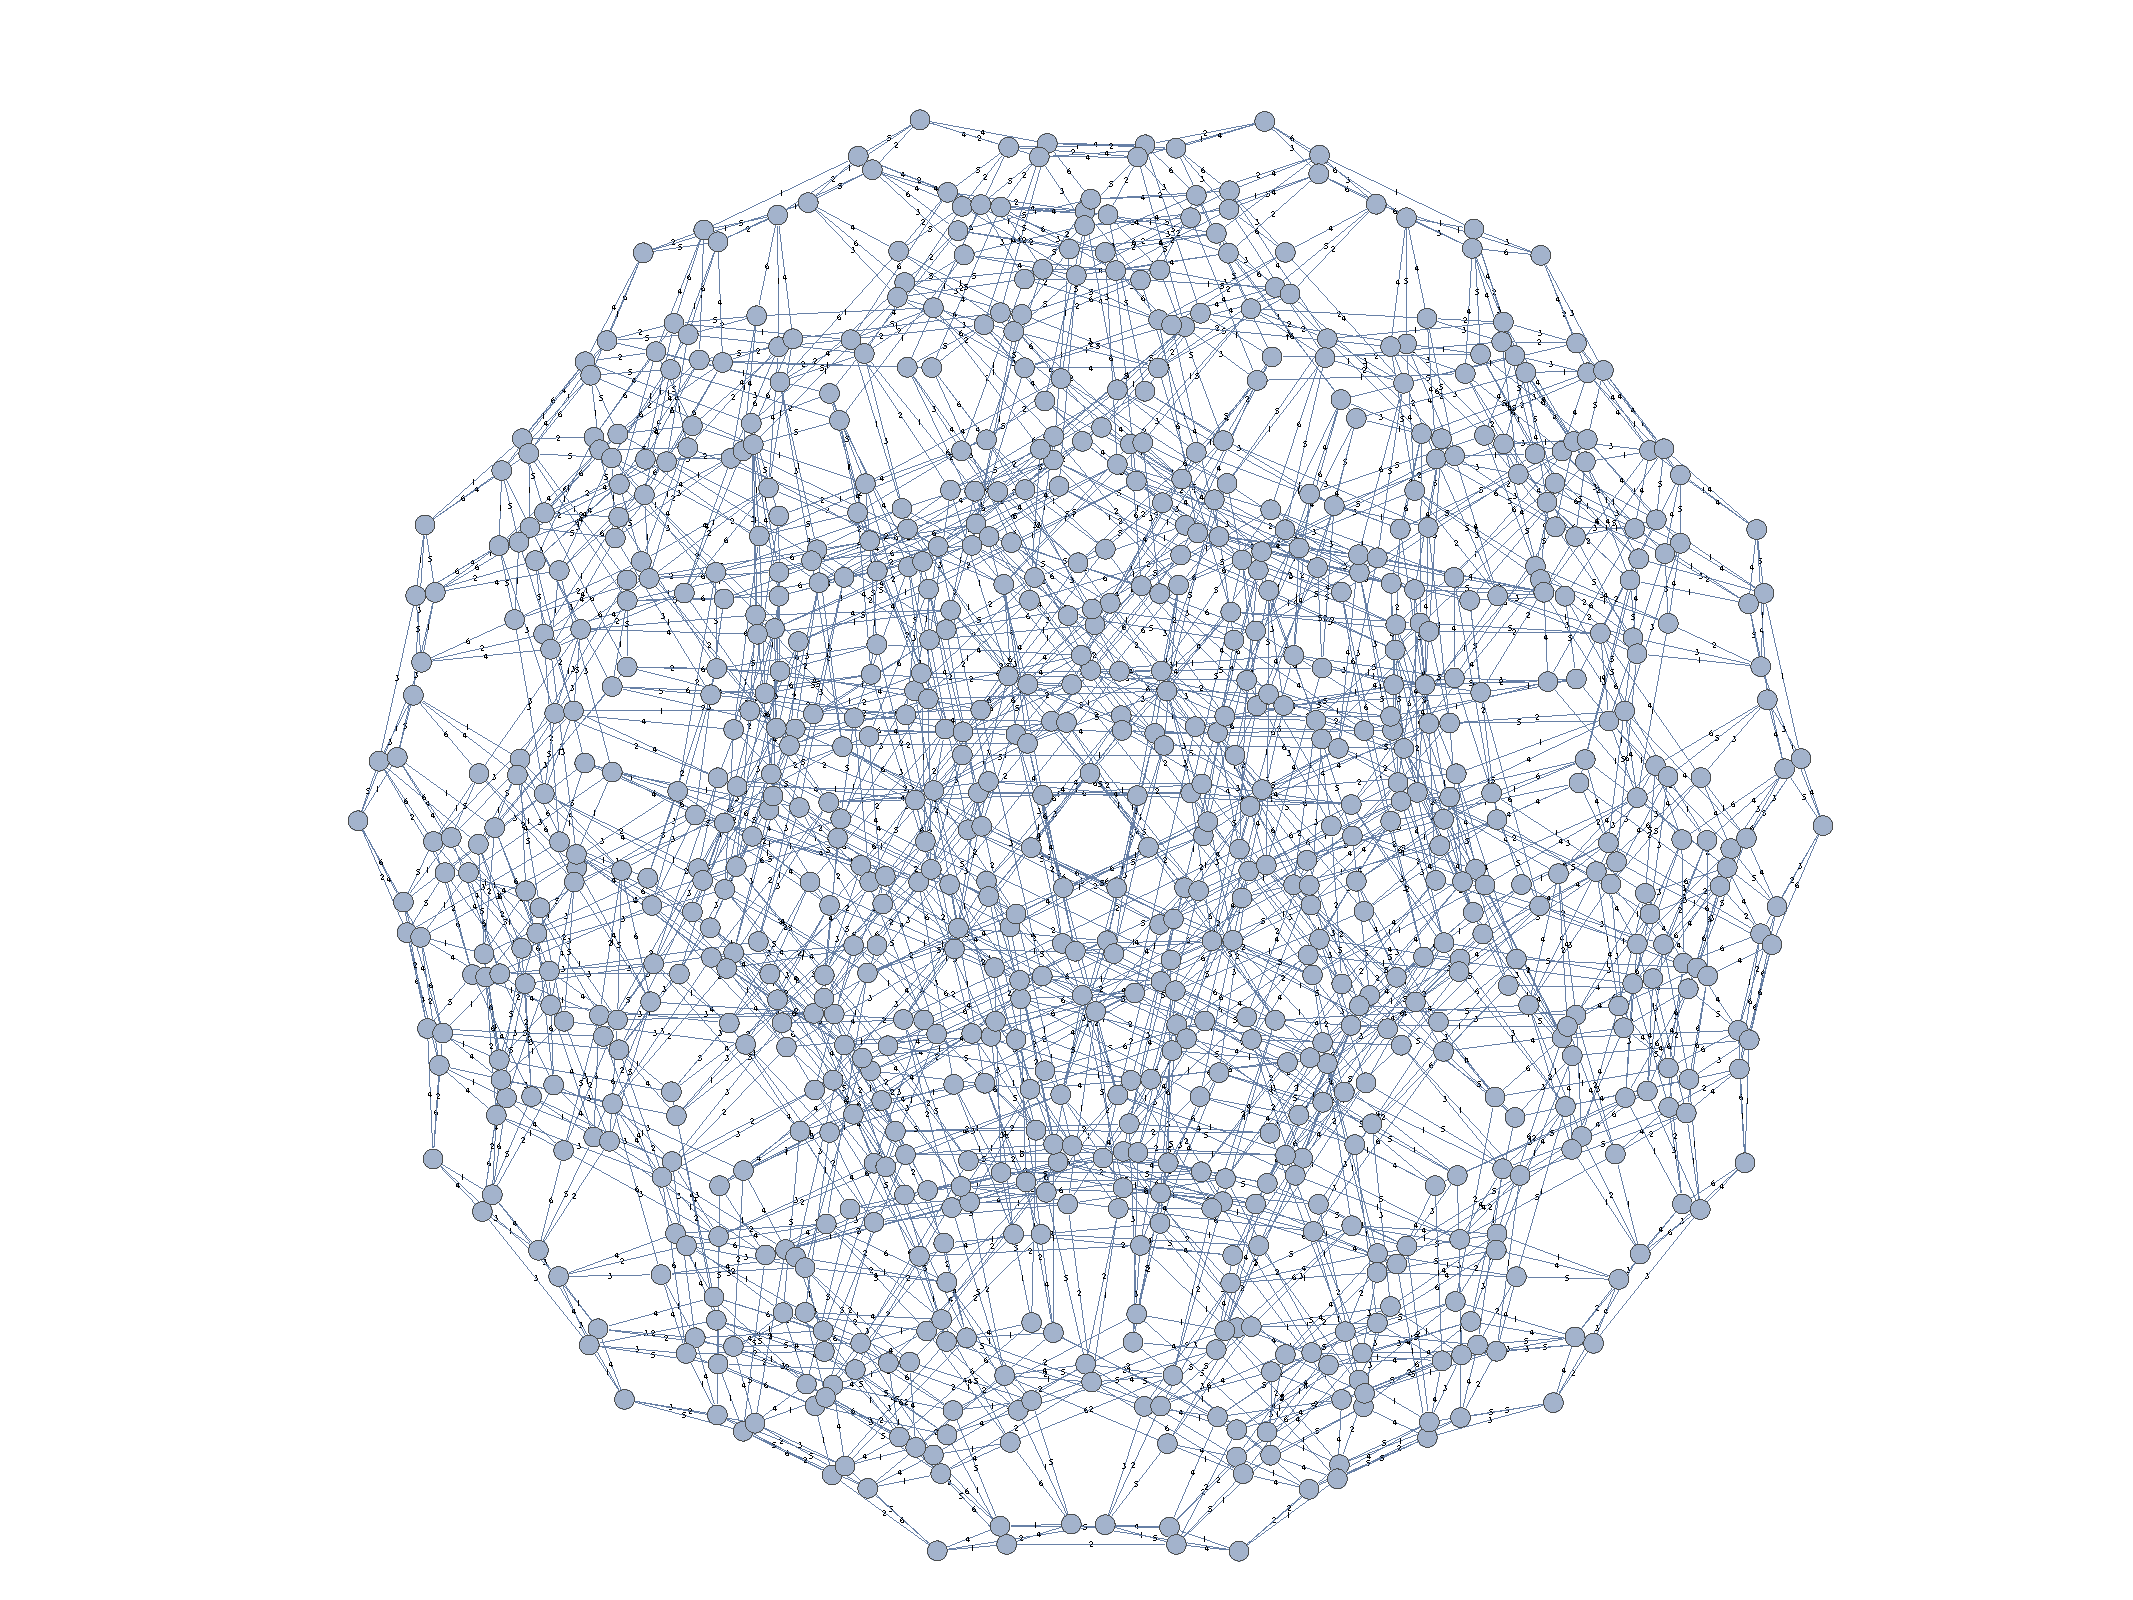
\includegraphics[scale=0.25]{e6-associahedron}
\end{figure}


\noindent It is not important to memorize any of this -- I just want to give you a flavor for the rich and complex structures that can arise from the simple mutation rules of eq. (\ref{eq:mutation})!

\section{Cluster \texorpdfstring{$\x$}{X}-coordinates}

Another important set of information encoded in cluster algebras are called Fock-Goncharov or $\x$-coordinates. Given a quiver described by the matrix $b$, the $\a$- and $\x$-coordinates are related as follows:
\begin{equation}
	x_i = \prod_j a_j^{b_{ij}}. 	
\end{equation} 
For example, the quiver 
\begin{equation}
\begin{gathered}
\begin{xy} 0;<1pt,0pt>:<0pt,-1pt>::
	(25,25) *+{\langle 13\rangle} ="0",
	(75,25) *+{\langle 14\rangle} ="1",
	(125,25) *+{\framebox[5ex]{$\langle 15\rangle$}} ="2",
	(125,75) *+{\framebox[5ex]{$\langle 45\rangle$}} ="3",
	(75,75) *+{\framebox[5ex]{$\langle 34\rangle$}} ="4",
	(25,75) *+{\framebox[5ex]{$\langle 23\rangle$}} ="5",
	(0,0) *+{\framebox[5ex]{$\langle 12\rangle$}} ="6",
	(145,75) *+{},
	"0", {\ar"1"},
	"4", {\ar"0"},
	"0", {\ar"5"},
	"6", {\ar"0"},
	"1", {\ar"2"},
	"3", {\ar"1"},
	"1", {\ar"4"},
\end{xy}
\end{gathered}
\end{equation}
has $\x$-coordinates 
\begin{equation}\label{def:xcoordsA2}
	\x_1 = \frac{\ket{12}\ket{34}}{\ket{14}\ket{23}}, \quad \x_2 = \frac{\ket{13}\ket{45}}{\ket{15}\ket{34}}.
\end{equation}
In the pentagon-triangulation picture, these $\x$-coordinates describe overlapping quadrilaterals:
\begin{center}
\begin{equation}
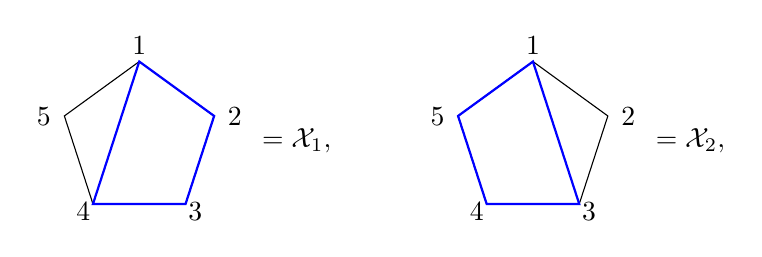
\begin{tikzpicture}
  \drawLabeledPentagon
  \draw[color=blue, thick] (P1) -- (P2) -- (P3) -- (P4) -- cycle;
  \draw (2,0) node {$=\x_1,$};
\begin{scope}[xshift = 5cm]
  \drawLabeledPentagon
  \draw[color=blue, thick] (P1) -- (P3) -- (P4) -- (P5) -- cycle;
  \draw (2,0) node {$=\x_2,$};
\end{scope}
\end{tikzpicture} 
\end{equation}
\end{center}
The nice feature of $\x$-coordinates, at least from a physicists perspective, is that in the case of $\Gr(4,n)$ the $\x$-coordinates are dual-conformal invariant cross-ratios. We can see this for example in the two-loop, six-particle remainder function for $\mathcal{N}=4$ SYM:
\begin{align}
	R^{(2)}_6 = &\sum_{\text{cyclic}} \text{Li}_4\left(-\frac{\langle 1234 \rangle \langle 2356 \rangle}{\langle 1236 \rangle \langle 2345 \rangle}\right) - \frac{1}{4} \text{Li}_4 \left(-\frac{\langle 1246 \rangle \langle 1345 \rangle}{\langle 1234 \rangle \langle 1456 \rangle}\right)\nl
	&+\text{products of } \text{Li}_{k}(-x) \text{ functions of lower weight}\\ &\quad~\text{with the same set of arguments.}\nn
\end{align}
The arguments of the polylogarithms all take the form of $(-\x)$-coordinates for $\Gr(4,6)$. $\x$-coordinates play other important roles in the context of polylogarithm functions independent of scattering amplitudes, for example with $\Gr(2,5) \leftrightarrow A_2$ we have 
\begin{equation}
	\sum_\text{cyclic} \Li_2(-\x_i) + \log(\x_i)\log(\x_{i+1}) = \frac{\pi^2}{6}
\end{equation}
where the definition of $\x_i$ can be inferred from eq. (\ref{def:xcoordsA2}). There are more complicated examples of polylogarithm identities satisfied by groups of $\x$-coordinates, for example there is a 40-term identity among $\Li_3$ functions where all of the arguments are $(-\x)$

Since we are motivated from physics to cast our final function-level results in terms of $\x$-coordinates it is useful to work entirely in that language rather than the $\a$-coordinates. The mutation rules for the $\x$-coordinates are
\begin{equation}
  \label{eq:x-coords-mutation}
  x_{i}' =
  \begin{cases}
    x_{k}^{-1}, &\quad i=k,\\
    x_{i} (1+x_{k}^{\sgn b_{i k}})^{b_{i k}}, &\quad i \neq k
  \end{cases},
\end{equation}
and the adjacency matrix $b_{ij}$ changes following eq.~(\ref{eq:b-mutation}). From here on out we will write our quivers entirely in terms of $\x$-coordinates, for example $A_2$ is 
\begin{equation}
	x_1 \to x_2.
\end{equation}
By continuing to mutate on alternating nodes (denoted below by \mbox{\color{red}{red}}) we generate the following sequence of clusters:
\begin{align}
  x_1 &\to \color{red}{x_2} \nl
  \color{red}{x_1(1+x_2)} &\leftarrow \frac{1}{x_2} \nl
  \frac{1}{x_1(1+x_2)} &\to \color{red}{\frac{x_2}{1+x_1+x_1 x_2}} \\
  \color{red}{\frac{x_1 x_2}{1+x_1}} &\leftarrow \frac{1+x_1+x_1 x_2}{x_2} \nl
  \frac{1+x_1}{x_1 x_2} &\to \color{red}{\frac{1}{x_1}} \nl
  \color{red}{x_2} &\leftarrow x_1 \nl
  &\vdots \nn
\end{align}
where the series then repeats. Note that by labeling the $\x$-coordinates as
\begin{equation}\label{def:a2-xcoords}
  \x_1 = 1/x_1, \quad \x_2 = x_2, \quad \x_3 = x_1(1+x_2), \quad 
  \x_4 = \frac{1+x_1+x_1 x_2}{x_2}, \quad \x_5 = \frac{1+x_1}{x_1 x_2},
\end{equation}
then the general mutation rule of eq. (\ref{eq:x-coords-mutation}) takes the simple form of
\begin{equation}\label{eq:exchange-relation}
  1+\x_i = \x_{i-1}\x_{i+1}.
\end{equation}
Putting this all together, we say that an $A_2$ cluster algebra is any set of clusters $1/\x_{i-1} \to \x_i$ for $i=1\ldots5$ where the $\x_i$ satisfy eq. (\ref{eq:exchange-relation}). We believe it is useful at this point to emphasize that one can take as input any $\{x_1, x_2\}$ and generate an associated $A_2$. For example, one could start with the quiver $3\to\frac{7}{2}$ and generate the $A_2$
\begin{equation}
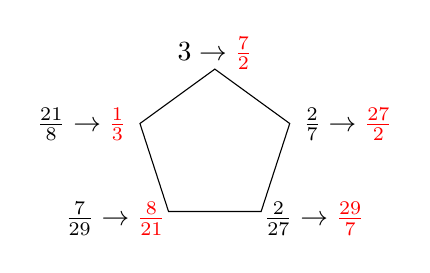
\begin{tikzpicture}
  \drawPentagon
  \draw (0,1.2) node {$3\to\color{red}{\frac{7}{2}}$};
  \draw (1,.3) node[anchor=west] {$\frac{2}{7} \to \color{red}{\frac{27}{2}} $};
  \draw (.5,-.9) node[anchor=west] {$\frac{2}{27} \to \color{red}{\frac{29}{7}}$};
  \draw (-.5,-.9) node[anchor=east] {$\frac{7}{29} \to \color{red}{\frac{8}{21}}$};
  \draw (-1,.3) node[anchor=east] {$\frac{21}{8} \to \color{red}{\frac{1}{3}}$};
\end{tikzpicture}
\end{equation}
(Mutating on the node in red moves you clockwise around the pentagon.) In future sections it will be necessary to consider collections of multiple $A_2$ algebras, in such cases we label them by only one of their clusters, e.g. $x_1 \to x_2$, with the understanding that we are referring to the $A_2$ which contains that cluster as an element. 

%This is all the information you need to start playing the cluster algebra game: write up some quiver and mutate away. A natural question is: will mutations always lead me to some closed set of clusters? The answer is that in general you will have infinite cluster algebras. The finite cluster %algebras were classified by Fomin and Zelevinsky \cite{} as relating to the Dynkin diagrams $A_n,~B_n,~C_n,$
%
%\section**{Grassmannian cluster algebras (and cluster Poisson spaces)}
%
%Let's now highlight why we might care about cluster algebras. There are two applications of particular relevance to scattering amplitudes. The first is %that the 5 $\x$-coordinates defined in eq. (\ref{def:a2-xcoords}) generate Abel's identity for the dilogarithm:
%\begin{equation}
	%\sum_{i=1}^5 \Li_2(-\x_i) \approx 0
%\end{equation}
%
%
%Unfortunately I have already managed to wildly mislead the reader and have presented a much different view of cluster algebras than most mathematicians (and mathematical physicists) would give. The core distinction is that there are two different ``coordinates'' one can use to describe cluster algebras: $\a$- and $\x$-coordinates, and most people work in terms of $\a$-coordinates. This is because the $\a$-coordinate representation of cluster algebras is actually a more broad and robust framework which contains the $\x$-coordinate representation in certain cases (in other words, you can go from $\a$%-coordinates to $\x$-coordinates, but not the other way around). 
%
%Fomin and Zelevinsky introduced cluster algebras in terms of $\a$-coordinates, and it was only later that Fock and Goncharov introduced the special case of $\x$-coordinates (they are often referred to as Fock-Goncharov coordinates, in fact). So why have I chosen to emphasize this more particular and limited framework? It is in large part because, as we will see, the cross-ratios that we amplitudeolog like to work with are $\x$-coordinates of certain cluster algebras. And so if our goal at the end of the day is to calculate physical quantities, $\x$-coordinates are likely going to be our core object %of focus, and it is often not necessary to invoke the full generality of $\a$-coordinates. 
%
%\begin{equation}
  %\label{eq:poisson-x-coords}
  %\lbrace x_{i}, x_{j}\rbrace = b_{i j} x_{i} x_{j}.
%\end{equation}
%
%\begin{equation}
  %\lbrace x_{i}', x_{j}'\rbrace = b_{i j}' x_{i}' x_{j}'
%\end{equation}
%
%\section*{Cluster polylogarithms and adjacency}
%
%\section*{Cluster automorphisms}
%Cluster algebras are often quite symmetric objects, and in cluster algberas with physical interpretations these symmetries frequently have a nice physical interpretation (e.g. Bose symmetry, etc). And of course these symmetries play many important roles in purely mathematical contexts, for example it turns out to be a natural and interesting problem to develop polylogarithm functions which share the same symmetries as various cluster algebras. In %this section we will 
%The simplest example of a cluster automorphism is what we will call a direct automorphism. Let $\a$ be a cluster algebra. Then $f: \a \to \a$ is direct %automorphism of $\a$ if
%\begin{itemize}
  %\item for every cluster $\mathbf{x}$ of $\a$, $f(\mathbf{x})$ is also a cluster of $\a$,
  %\item $f$ respects mutations, i.e. $f(\mu(x_i,\mathbf{x})) = \mu(f(x_i),f(\mathbf{x}))$.
 %\end{itemize} 
%A simple example of this for $A_2$ is the map
%\begin{equation}
  %\sigma_{A_2}:\quad \x_i \mapsto \x_{i+1},
%\end{equation}
%which cycles the five clusters $1/\x_i\to \x_{i+1}$ amongst themselves, and can be cast in terms of the seed variables $x_1, x_2$ as 
%\begin{equation}
  %\sigma_{A_2}:\quad x_1\mapsto \frac{1}{x_2},~~ x_2\mapsto x_1(1+x_2).
%\end{equation}
%
%A less obvious example of a cluster automorphism is what we will call an indirect automorphism, which respect mutations but do not map clusters directly %on to clusters; instead
%\begin{itemize}
  %\item for every cluster $\mathbf{x}$ of $\a$, $f(\mathbf{x})$ + invert all nodes + swap direction of all arrows\\ = a cluster of $\a$.
%\end{itemize}
%For $A_2$ we have the indirect automorphism
%\begin{equation}
  %\tau_{A_2}:\quad \x_i \mapsto \x_{6-i},
%\end{equation}
%where indices are understood to be mod 5, and can instead be cast in terms of the seed variables $x_1, x_2$ as
%\begin{equation}
  %\tau_{A_2}:\quad x_1 \to \frac{1}{x_2}, ~~x_2 \mapsto \frac{1}{x_1}.
%\end{equation}
%We can see how this works in a simple example
%\begin{align}
  %\tau_{A_2}(1/\x_1 \to \x_2) =&~1/\x_5 \to \x_4 \nl
  %\Rightarrow &\text{ invert each node and swap direction of all arrows }\\ 
  %=&~\x_5 \leftarrow 1/\x_4, \text{ which is in our original $A_2$}.\nn
%\end{align}
%It is useful to think of indirect automorphisms as generating a ``mirror'' or ``flipped'' version of the original $\a$, where the total collection of $\x$-coordinates is the same, but their Poisson bracket has flipped sign. The existence of this flip then can be seen as resulting from the choice of assigning $b_{ij}$ = (\# arrows $i\to j$) - (\# arrows $j \to i$), where instead we could have chosen $b_{ij}$ = (\# arrows $j \to i$) - (\# arrows $i\to j$) and still generated the same clsuter algebraic structure, albeit with different labels for the nodes. In the generic case this is an arbitrary %choice, and $\tau$ captures the superficiality of the notation change.
%
%The automorphisms $\sigma_{A_2}$ and $\tau_{A_2}$ generate the complete automorphism group for $A_2$, namely, $D_5$ (the notation here is regretably redundant; here we are referring to the dihedral group of five elements, which is of course distinct from the Dynkin diagram $D_5$ -- we hope that context will clarify to the reader what we mean in each case). In the appendix~\ref{appendix:automorphisms} we list generators for the automorphism %groups of several relevant (finite) cluster algebras. 
%
%
%
%
%%\begin{tikzpicture}
%%  \drawPentagon
%%  \foreach \a/\l in {90/1,18/2,306/3,234/4,162/5} {
%%    \coordinate (P\l) at (\a:1cm); 
%%    \node[anchor=\a] at ($(P\l)+(\a+0:.5cm)$) {\l};
%%  }
%%  \draw[color=red] (P1) -- (P3);
%%  \draw[color=red] (P1) -- (P4);
%%\end{tikzpicture}
%
%\section*{The \texorpdfstring{$A_2$}{A2} function}
%We define the $A_2$ function as
%\begin{equation}
	%f_{A_2}  = \sum_{\text{skew-dihedral}} f_i^\pm = \sum_{i=1}^5 ( f_i^+ - f_i^- ) 
%\end{equation}
%in terms of the building blocks
%\begin{equation}
%f^\pm_{i}=\Li_{2,2}(-x_i,-x_{i\pm2})-\Li_{1,3}(-x_i,-x_{i\pm2})-\Li_2(-x_i)\log(x_{i\pm1})\log(x_{i\pm2}).
%\end{equation}
%where $6-i$ is understood to be mod 5. It has the symbol
%\begin{align}
   %-\sum_{\text{skew-dihedral}}
   %&x_i \otimes x_i \otimes x_{i+1} \otimes x_{i+1}
   %+x_i \otimes x_{i+1} \otimes x_i \otimes x_{i-1}
   %+x_i \otimes x_{i+1} \otimes x_{i+1} \otimes x_i\\
   %&\quad-2\left(x_i \otimes x_{i+1} \otimes (x_ix_{i+2}) \otimes x_{i+1}
   %-x_i \otimes x_{i+1} \otimes x_{i+1} \otimes x_{i+2}\right)\nl
%\end{align}
%
%\begin{align}
   %-\sum_{\text{skew-dihedral}}
   %&[i , i , i+1 , i+1]
   %+[i , i+1 , i , i-1]
   %+[i , i+1 , i+1 , i]\\&-2\left([i , i+1 , (ii+2) , i+1]
   %-[i , i+1 , i+1 , i+2]\right)
%\end{align}
%
%\begin{equation}
   %-\sum_{\text{skew-dihedral}}[1122]+[1215]+[1221]-2([1212]+[1232]-[1223])
%\end{equation}
%
%And satisfies the properties:
%\begin{itemize}
   %\item clustery cobracket
   %\item cluster adjacent in $A_2$
   %\item smooth and real-valued in the positive domain
%\end{itemize}
%
%\section*{Cluster subalgebra-constructibility and the \texorpdfstring{$A_3$}{A3} function}
%
%\section*{Previous applications for 6- and 7-pt amplitudes}
%
%\appendix
%
%\section*{Automorphisms}\label{appendix:automorphisms}
%
%See \cite{Chang:2015} for a more thorough mathematical introduction. 
%
%Cluster algebras of type $A_n \simeq \Gr(2,n+3)$ 
%\begin{equation}
  %x_1\to x_2\to \ldots \to x_n
%\end{equation}
%have automorphism group $D_{n+3}$, with a cyclic generator $\sigma_{A_n}$ (direct, length $n+3$)
%\begin{equation}
  %\sigma_{A_n}:\quad x_{k<n} \mapsto \frac{x_{k+1}(1+x_{1,\ldots,k-1})}{1+x_{1,\ldots,k+1}},~~x_n\mapsto\frac{1+x_{1,\ldots,n-1}}{\prod_{i=1}^n x_i}
%\end{equation}
%and flip generator $\tau_{A_n}$ (indirect)
%\begin{equation}
  %\tau_{A_n}: \quad x_1 \mapsto \frac{1}{x_n},~~x_2 \mapsto \frac{1}{x_{n-1}},~\ldots~,x_n\mapsto\frac{1}{x_1}.
%\end{equation}
%
%The cluster algebra $D_4 \simeq \Gr(3,6)$
%\begin{equation}
    %\begin{gathered}
    %\begin{xy} 0;<1pt,0pt>:<0pt,-1pt>::
      %(0,20) *+{x_1} ="1",
      %(30,20) *+{x_2} ="2",
      %(60,0) *+{x_3} ="3",
      %(60,40) *+{x_4} ="4",
      %"1", {\ar"2"},
      %"2", {\ar"3"},
      %"2", {\ar"4"},
    %\end{xy}
    %\end{gathered}
%\end{equation}
%has automorphism group $D_4\times S_3$, with two cyclic generators: 
%\begin{equation}
%\begin{split}
  %\sigma^{(4)}_{D_4}:\quad& 
    %x_1\mapsto\frac{x_2}{1+x_{1,2}},~~  
    %x_2\mapsto\frac{\left(1+x_1\right)x_1 x_2 x_3 x_4}{\left(1+x_{1,2,3}\right) \left(1+x_{1,2,4}\right)},~~
    %x_3\mapsto\frac{1+x_{1,2}}{x_1 x_2 x_3},~~
    %x_4\mapsto\frac{1+x_{1,2}}{x_1 x_2 x_4},\\ \\
  %\sigma^{(3)}_{D_4}:\quad& 
    %x_1\mapsto \frac{1}{x_3},~~
    %x_2\mapsto \frac{x_1 x_2 \left(1+x_3\right)}{1+x_1},~~
    %x_3\mapsto x_4,~~
    %x_4\mapsto \frac{1}{x_1},
%\end{split}  
%\end{equation}
%where $\sigma^{(4)}_{D_4}$ generates the 4-cycle and $\sigma^{(3)}_{D_4}$ the 3-cycle in $D_4$ and $S_3$, respectively. Then there is the indirect $\tau$%-flip associated with the $D_4$ automorphism, as well as a direct $\mathbb{Z}_2$-flip associated with the $S_3$ automorphism:
%\begin{equation}
%\begin{split}
  %\tau_{D_4}:\quad& 
    %x_2\mapsto \frac{1+x_1}{x_1 x_2 \left(1+x_3\right) \left(1+x_4\right)},\\ \\
  %\mathbb{Z}_{2,D_4}:\quad& 
    %x_3\mapsto x_4,~~
    %x_4\mapsto x_3.
%\end{split}  
%\end{equation}
%The cluster algebra $D_{n>4}$
%\begin{equation}
    %\begin{gathered}
    %\begin{xy} 0;<1pt,0pt>:<0pt,-1pt>::
      %(0,20) *+{x_1} ="1",
      %(30,20) *+{x_2} ="2",
      %(60,20) *+{\ldots} ="3",
      %(90,20) *+{x_{n-2}} ="4",
      %(120,0) *+{x_{n-1}} ="5",
      %(120,40) *+{x_{n}} ="6",
      %"1", {\ar"2"},
      %"2", {\ar"3"},
      %"3", {\ar"4"},
      %"4", {\ar"5"},
      %"4", {\ar"6"},
    %\end{xy}
    %\end{gathered}
%\end{equation}
%has automorphism group $D_n \times \mathbb{Z}_2$ with generators $\sigma_{D_n}$ ($n$-cycle, direct), $\mathbb{Z}_{2,D_n}$ (2-cycle, direct), and $\tau_{D%_n}$ (2-cycle, indirect). The $Z_2$ simply swaps $x_{n-1} \leftrightarrow x_n$, and for $D_5$ the $\sigma$ and $\tau$ generators can be represented by
%\begin{equation}
%\begin{split}
  %\sigma_{D_5}:\quad& 
    %x_1\mapsto \frac{x_2}{1+x_{1,2}},~~
    %x_2\mapsto \frac{(1+x_1) x_3}{1+x_{1,2,3}},~~
    %x_3\mapsto \frac{x_1 x_2 x_3 x_4 x_5 (1+x_{1,2})}{(1+x_{1,2,3,4}) (1+x_{1,2,3,5})},\\&
    %x_4\mapsto \frac{1+x_{1,2,3}}{x_1 x_2 x_3 x_4},~~
    %x_5\mapsto \frac{1+x_{1,2,3}}{x_1 x_2 x_3 x_5},\\ \\
  %\tau_{D_5}:\quad& 
    %x_1\mapsto x_1,~~
    %x_2\mapsto \frac{1+x_1}{x_1 x_2 (1+x_3 x_5+x_{3,4,5})},~~
    %x_3\mapsto \frac{x_3 x_4 x_5}{(1+x_{3,4}) (1+x_{3,5})},\\&
    %x_4\mapsto \frac{1+x_3 x_5+x_{3,4,5}}{x_4},~~
    %x_5\mapsto \frac{1+x_3 x_5+x_{3,4,5}}{x_5}.
%\end{split}  
%\end{equation}
%Finally, we describe the cluster algebra $E_6 \simeq \Gr(4,7)$
%\begin{equation}
    %\begin{gathered}
    %\begin{xy} 0;<1pt,0pt>:<0pt,-1pt>::
      %(0,0) *+{x_1} ="1",
      %(30,0) *+{x_2} ="2",
      %(60,0) *+{x_3} ="3",
      %(60,-25) *+{x_4} ="4",
      %(90,0) *+{x_5} ="5",
      %(120,0) *+{x_5} ="6",
      %"1", {\ar"2"},
      %"2", {\ar"3"},
      %"4", {\ar"3"},
      %"5", {\ar"3"},
      %"6", {\ar"5"},
    %\end{xy}
    %\end{gathered}
%\end{equation}
%which has automorphism group $D_{14}$ with generators $\sigma_{E_6}$ (7-cycle, direct), $\mathbb{Z}_{2,E_6}$ (2-cycle, direct), and $\tau_{E_6}$ (2-cycle, indirect). In $\Gr(4,7)$ language, these are the traditional cycle ($Z_i \to Z_{i+1}$), parity ($Z \to W$'s), and flip ($Z_i \to Z_{8-i}$) %symmetries, respectively. In $E_6$ langauge they can be represented by 
%\begin{equation}
%\begin{split}
  %\sigma_{E_6}:\quad& 
    %x_1\mapsto \frac{1}{x_6 (1+x_{5,3,4})},~~
    %x_2\mapsto \frac{1+x_{6,5,3,4}}{x_5 (1+x_{3,4})},~~
    %x_3\mapsto \frac{(1+x_{2,3,4}) (1+x_{5,3,4})}{x_3 (1+x_4)},\\&
    %x_4\mapsto \frac{1+x_{3,4}}{x_4},~~
    %x_5\mapsto \frac{1+x_{1,2,3,4}}{x_2 (1+x_{3,4})},~~
    %x_6\mapsto \frac{1}{x_1 (1+x_{2,3,4})},\\ \\
  %\mathbb{Z}_{2,E_6}:\quad& 
    %x_i\mapsto x_{7-i},\\ \\
  %\tau_{E_6}:\quad& 
    %x_1\mapsto \frac{x_5}{1+x_{6,5}},~~
    %x_2\mapsto (1+x_5) x_6,~~
    %x_3\mapsto \frac{(1+x_{1,2}) (1+x_{6,5})}{x_1 x_2 x_3 x_5 x_6 (1+x_4)},\\&
    %x_4\mapsto x_4,~~
    %x_5\mapsto x_1 (1+x_2),~~
    %x_6\mapsto \frac{x_2}{1+x_{1,2}}.
%\end{split}  
%\end{equation}
%
%
%
%
%
\bibliographystyle{ieeetr}

\bibliography{motives44}

\end{document}
